%-------------------------------------------------------------
\subsection{Example 3} \label{sec:ch5:example3}

%-------------------------------------------------------------
\subsubsection{Description}

For the third example, we will consider the problem on pp.~109--110 of Ref.~\cite{Bryson1975a}:
\begin{subequations}%%
\begin{align}
\min_{u(t)} \quad & \frac{a^2}{2} [ \xi(t_f) ]^2 + \frac{1}{2}\int_{0}^{t_f} u^2 dt \\
\text{subject to:} \quad  & \dot{\xi} = b(t) u \\
& \xi(0) = \xi_0 \\
& \abs{u(t)} \leq 1
\end{align}
\end{subequations}%

\noindent This problem has time-varying matrices, path constraints, and both Lagrange and Mayer terms.
The structure-based problem description for this example is:
\allowdisplaybreaks[1]%
\begin{subequations}%%
\begin{gather}
% Mayer term
\mathcal{M}\xind{1}.\xvar{left} = 5, \quad \mathcal{M}\xind{1}.\xvar{right} = 5, \quad \mathcal{M}\xind{1}.\xvar{matrix} = a^2/2 \\
% Lagrange term
\mathcal{L}\xind{1}.\xvar{left} = 1, \quad \mathcal{L}\xind{1}.\xvar{right} = 1, \quad \mathcal{L}\xind{1}.\xvar{matrix} = 1/2 \\
% dynamics
A = 0, \quad B = b(t) \\
% initial condition
% simple bound
\mathcal{UB}\xind{1}.\xvar{right} = 4, \quad \mathcal{UB}\xind{1}.\xvar{matrix} = \xi_0, \quad
\mathcal{LB}\xind{1}.\xvar{right} = 4, \quad \mathcal{LB}\xind{1}.\xvar{matrix} = \xi_0 \\
\mathcal{UB}\xind{2}.\xvar{right} = 1, \quad \mathcal{UB}\xind{2}.\xvar{matrix} = 1, \quad
\mathcal{LB}\xind{2}.\xvar{right} = 1, \quad \mathcal{LB}\xind{2}.\xvar{matrix} = -1
\end{gather}
\end{subequations}%%
\allowdisplaybreaks[0]%

\noindent The \textsc{Matlab} code is in Sec.~\ref{sec:ex3-code}.

%-------------------------------------------------------------
\subsubsection{Solution}

\begin{figure}
\centering

\begin{subfigure}{0.5\textwidth}
\centering
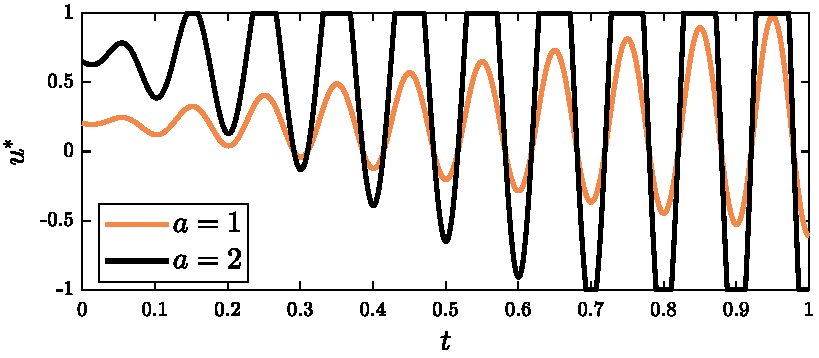
\includegraphics[width=\textwidth]{../ch5/figures/ex3sol-controls}%
\caption{Control.}
\label{fig:ch5:ex3sol:controls}
\end{subfigure}%
\begin{subfigure}{0.5\textwidth}
\centering
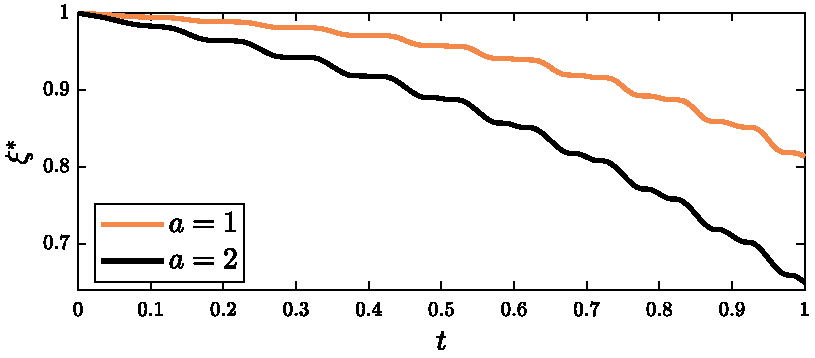
\includegraphics[width=\textwidth]{../ch5/figures/ex3sol-states}%
\caption{State.}
\label{fig:ch5:ex3sol:states}
\end{subfigure}%

\caption{Solutions for \nameref{sec:ch5:example3}.}
\label{fig:ch5:ex3sol}
\end{figure}

The optimal control is:
\begin{align}
u^*(t) &= - \mathrm{sat}\left[ a^2 b(t) \xi(t_f) \right]
\end{align}

\noindent where $\xi(t_f)$ is computed from the implicit equation:
\begin{align}
\xi(t_f) &= \xi_0 - \int_0^{t_f} b(t) \mathrm{sat}\left[ a^2 b(t) \xi(t_f) \right] dt 
\end{align}

\noindent The problem parameters used are $t_f = 1$, $\xi_0 = 1$, and $b(t) = t \cos(20 \pi t) - 1/4$.
Both $a = 1$ and $a = 2$ will be tested.
For $a=1$, $\Psi^* = 0.406759$ and $\xi^*(t_f) = 0.813517$.
For $a=2$, $\Psi^* = 1.150647$ and $\xi^*(t_f) = 0.649528$.
The optimal trajectories for control and state for both values of $a$ are shown in Fig.~\ref{fig:ch5:ex3sol}.
With $a=1$, the path constraints are never active, but with $a=2$, the path constraints switch activity frequently. 

%-------------------------------------------------------------
\subsubsection{Numerical Results}

\begin{figure}%
\centering

{\footnotesize Local maximum values (local minimum values are in a thinner, translucent color):}


\includegraphics[width=\textwidth]{../ch5/figures/ex1_sens_legend}%

\vspace{1mm}

\begin{subfigure}{0.5\textwidth}
\centering
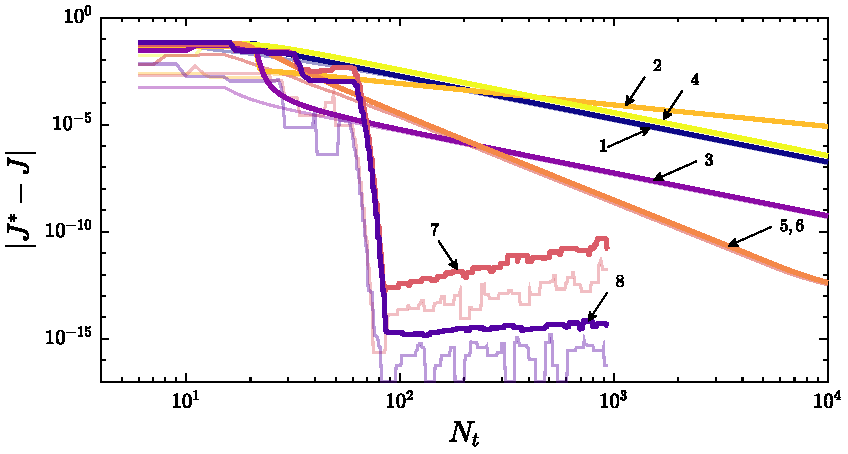
\includegraphics[width=\textwidth]{../ch5/figures/ex3_sens_objective_a1}%
\caption{Objective error with $a=1$.}
\label{fig:ch5:ex3sens:objective:a1}
\end{subfigure}%
\begin{subfigure}{0.5\textwidth}
\centering
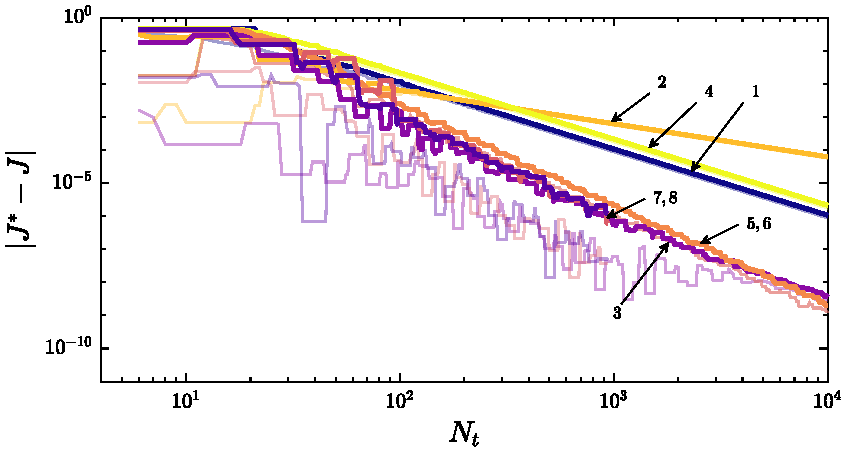
\includegraphics[width=\textwidth]{../ch5/figures/ex3_sens_objective_a2}%
\caption{Objective error with $a=2$.}
\label{fig:ch5:ex3sens:objective:a2}
\end{subfigure}%

\begin{subfigure}{0.5\textwidth}
\centering
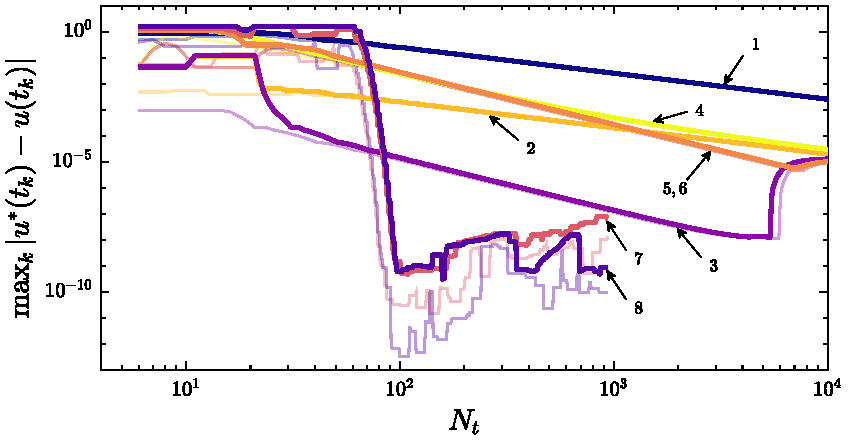
\includegraphics[width=\textwidth]{../ch5/figures/ex3_sens_control_a1}%
\caption{Control error with $a=1$.}
\label{fig:ch5:ex3sens:control:a1}
\end{subfigure}%
\begin{subfigure}{0.5\textwidth}
\centering
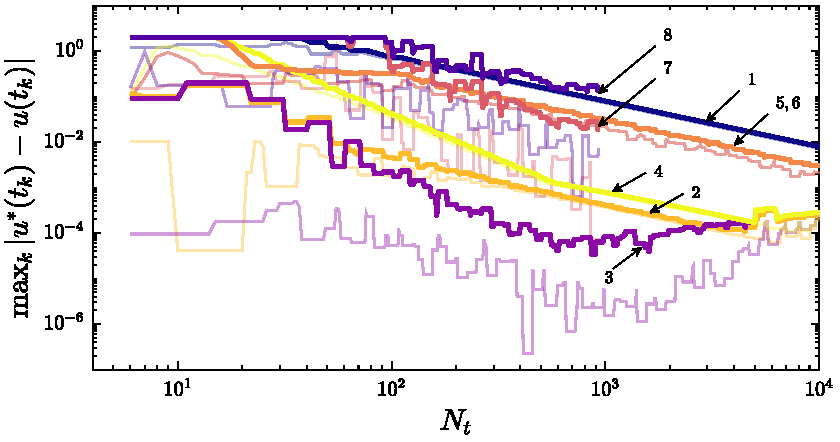
\includegraphics[width=\textwidth]{../ch5/figures/ex3_sens_control_a2}%
\caption{Control error with $a=2$.}
\label{fig:ch5:ex3sens:control:a2}
\end{subfigure}%

\begin{subfigure}{0.5\textwidth}
\centering
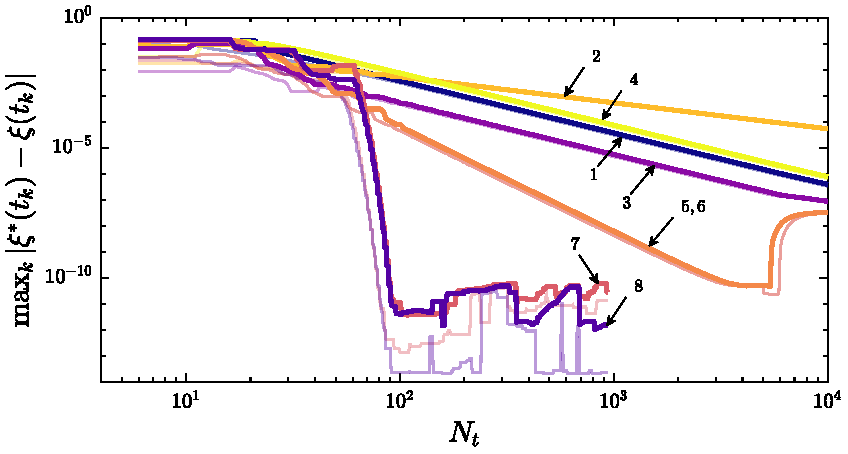
\includegraphics[width=\textwidth]{../ch5/figures/ex3_sens_state_1_a1}%
\caption{State error with $a=1$.}
\label{fig:ch5:ex3sens:state:a1}
\end{subfigure}%
\begin{subfigure}{0.5\textwidth}
\centering
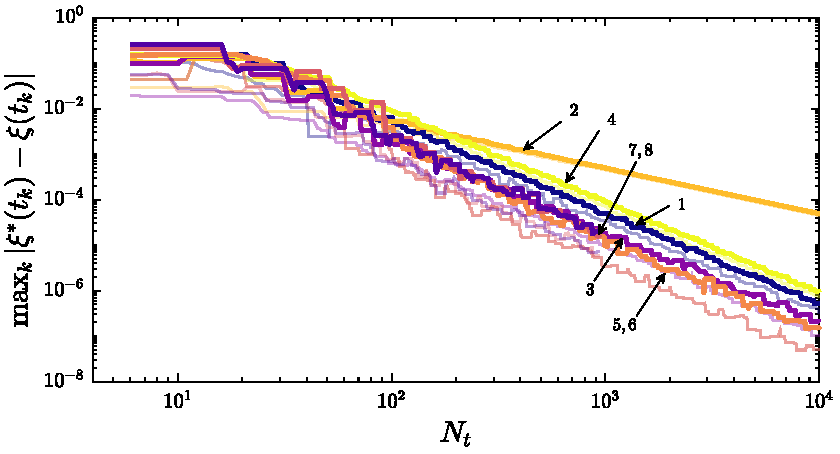
\includegraphics[width=\textwidth]{../ch5/figures/ex3_sens_state_1_a2}%
\caption{State error with $a=2$.}
\label{fig:ch5:ex3sens:state:a2}
\end{subfigure}%

\caption{Numerical results for \nameref{sec:ch5:example3}.}
\label{fig:ch5:ex3sens}
\end{figure}

The convergence results for the eight tested schemes and both values of $a$ are shown in Fig.~\ref{fig:ch5:ex3sens}.
When $a=1$ (where the path constraints are not active), the results are somewhat similar to \nameref{sec:ch5:example1}.
The best methods are the two PS-based schemes (7,8), but unlike the previous example, the gap between them is negligible.
Although the SS-based schemes are converging to the true solution, the ranking of the schemes depends highly on the relative preference between the objective, control, or state errors.
The two CQHS-based schemes have lower state error, but higher control error.
ED-TR-CTR (3) has much lower control error, but higher state error. 
With respect to the objective error, (3) begins with lower error but there is a transition point around $N_t=200$ where (5,6) exhibit less error.
We also see ED-HS-CTR (4) performing worse than (3), differing from the previous examples.

% new paragraph
With $a=2$, the results are quite different with more sporadic convergence behavior (especially for the control).
We observe that (3) is now the best scheme.
Combining the results from both values of $a$, (3) appears to be the best option if high accuracy is required in both problem versions.
These unexpected results might be explained by the fact that there is no $\bm{A}$ in this example (a fairly uncommon property in \lqdo).
As a result, this example may prove to be a useful, challenging test problem in the future.
Fully understanding these results is left as future work.